\section{Durchführung}
Das Kernstück des Versuchsaufbaus ist eine transparente Grundplatte, auf der sich zwei Laser befinden. 
Der obere laser strahlt in rot bei einer Wellenlänge von $\lambda = \qty{635}{\nano\meter}$ während der
untere laser ein grünes licht mit der Wellenlänge $\lambda = \qty{532}{\nano\meter}$ ausstrahlt.
Laser stahlen auf den Mittelpunkt eines Halbkreises, auf dem sie sich bewegen können.
Je nach Versuch wird dort ein optisches Element platziert.
Unter der Grundplatte liegt eine Schablone, die zum ablesen der Ein- und Austrittswinkel der optischen
Elemente geeignet ist.
\begin{figure}
    \centering
    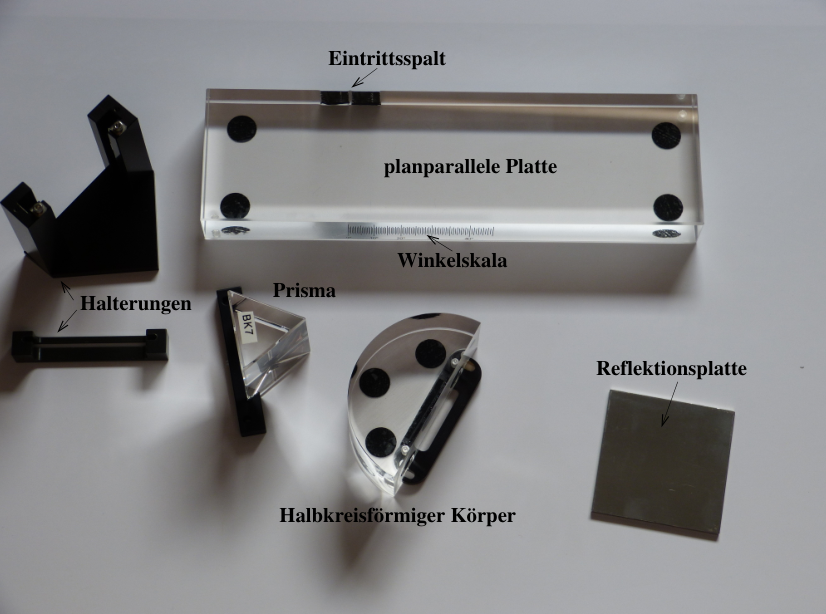
\includegraphics{Abbildungen/Aufbau.png}
    \caption{Der Aufbau des Versuchs ohne optisches Element \cite{man:v400}.}
\end{figure}

\subsection{Reflexionsgesetz}
Für die Messung des Reflexionsgesetzes wird ein Laser im Winkel
$\alpha_1$ auf einen Spiegel gehalten (für Winkelbezeichnungen vgl. Abbildung \ref{fig:teo_refl_brech}).
Der Austrittswinkel $\alpha_2$ des Lasers wird für 7 Einfallswinkel mithilfe der Schablone abgelesen und notiert.

\subsection{Brechungsgesetz und Strahlversatz}
Für diesen Versuch wird als optisches Element ein Plexiglasblock der tiefe $d = \qty{5.85}{\cm}$ eingesetzt.
der laser Strahlt auf einen schmalen nicht abgedunkelten Spalt auf der Oberfläche Des Blocks.
Auf der gegenüberliegenden Seite des Blocks ist eine Skala für den Brechungswinkel $\beta$ eingetragen.
Für $m= 7$ Einfallswinkel $\alpha$ wird $\beta$ notiert.
Der Strahlversatz wird mithilfe von Gleichung \eqref{eq:teo_strahlversatz} berechnet.
Zum einen wird der Winkel $\beta$ mithilfe des Brechungsgesetzes berechnet,
zum anderen werden die gemessenen Winkel $\beta$ in der Formel verwendet.
%% Was ist was (s_1 und s_2)?

\subsection{Prisma}
An dem Prisma werden... 




\subsection{Beugung am Gitter}
Die beiden Laserstahlen werden gerade auf Gitter mit \num{600}, \num{300} und \num{100} Linien/\unit{\mm} gehalten.
mit einer Schablone werden die Winkel der Maxima des Beugungsmusters abgelesen un notiert.